\documentclass[11pt]{article}

% ------------------------------------------------------------------------------
% This is all preamble stuff that you don't have to worry about.
% Head down to where it says "Start here"
% ------------------------------------------------------------------------------

\usepackage[margin=.8in,top=1.1in,bottom=1.1in]{geometry} % page layout
\usepackage{amsmath,amsthm,amssymb,amsfonts} % math things
\usepackage{graphicx} % include graphics
\usepackage{fancyhdr} % header customization
\usepackage{titlesec} % help with section naming
\usepackage{listings}
\usepackage[final]{pdfpages}

% naming sections
\titleformat{\section}{\bf}{Problem \thesection}{0.5em}{}
\newcommand{\exercise}{\section{}}

% headers
\pagestyle{fancy}
\fancyhf{} % clear all
\fancyhead[L]{\sffamily\small Machine Learning 1 --- Homework}
\fancyhead[R]{\sffamily\small Page \thepage}
\renewcommand{\headrulewidth}{0.2pt}
\renewcommand{\footrulewidth}{0.2pt}
\markright{\hrulefill\quad}

\newcommand{\hwhead}[4]{
\begin{center}
\sffamily\large\bfseries Machine Learning Worksheet #1
\vspace{2mm}
\normalfont

#2\\
#3\\
\texttt{#4}
\end{center}
\vspace{6mm} \hrule \vspace{4mm}
}

% ------------------------------------------------------------------------------
% Start here -- Fill in your name, imat and email
% (and the same for who you worked with)
% You are allowed to work in groups of 2 (or 3 if there is no way around it)
% However, you each must submit individually - (it may be same file)
% ------------------------------------------------------------------------------

\newcommand{\names}{Tomas Ladek, Michael Kratzer} %
\newcommand{\imats}{3602673, 3612903} %
\newcommand{\emails}{tom.ladek@tum.de, mkratzer@mytum.de} %

\begin{document}

% ------------------------------------------------------------------------------
% Change xx (and only xx) to the current sheet number
% ------------------------------------------------------------------------------
\hwhead{8}{\names}{\imats}{\emails}

% ------------------------------------------------------------------------------
% Fill in your solutions
% ------------------------------------------------------------------------------

\exercise
\begin{align*}
	\nabla E(w) = \begin{pmatrix}
		\frac{\partial E(w)}{\partial w_1} \\
		\vdots \\
		\frac{\partial E(w)}{\partial w_d}
	\end{pmatrix}
\end{align*}
with
\begin{align*}
	\frac{\partial E(w)}{\partial w_i} = \frac{1}{m}\sum_{i=1}^{m}f'(z_i -wx_i)x_i + \gamma w_i \\
	f'(x) = \begin{cases}
		x  & |x|<1 \\
		sgn(x) & otherwise
	\end{cases}
\end{align*}

\exercise
To minimize the error or loss we have to find better values for the weights w. This is normaly not a convex problem so we have to use an incremental approach like steepest decent to propagate changes back through the network and adjusting the weights.
\begin{align}
	w_{i+1} = w_i - \alpha \nabla E(w)
\end{align}
$\alpha$ is the learing rate.

\exercise
Only implementation in the perceptron example, but it does not seem to be correct.
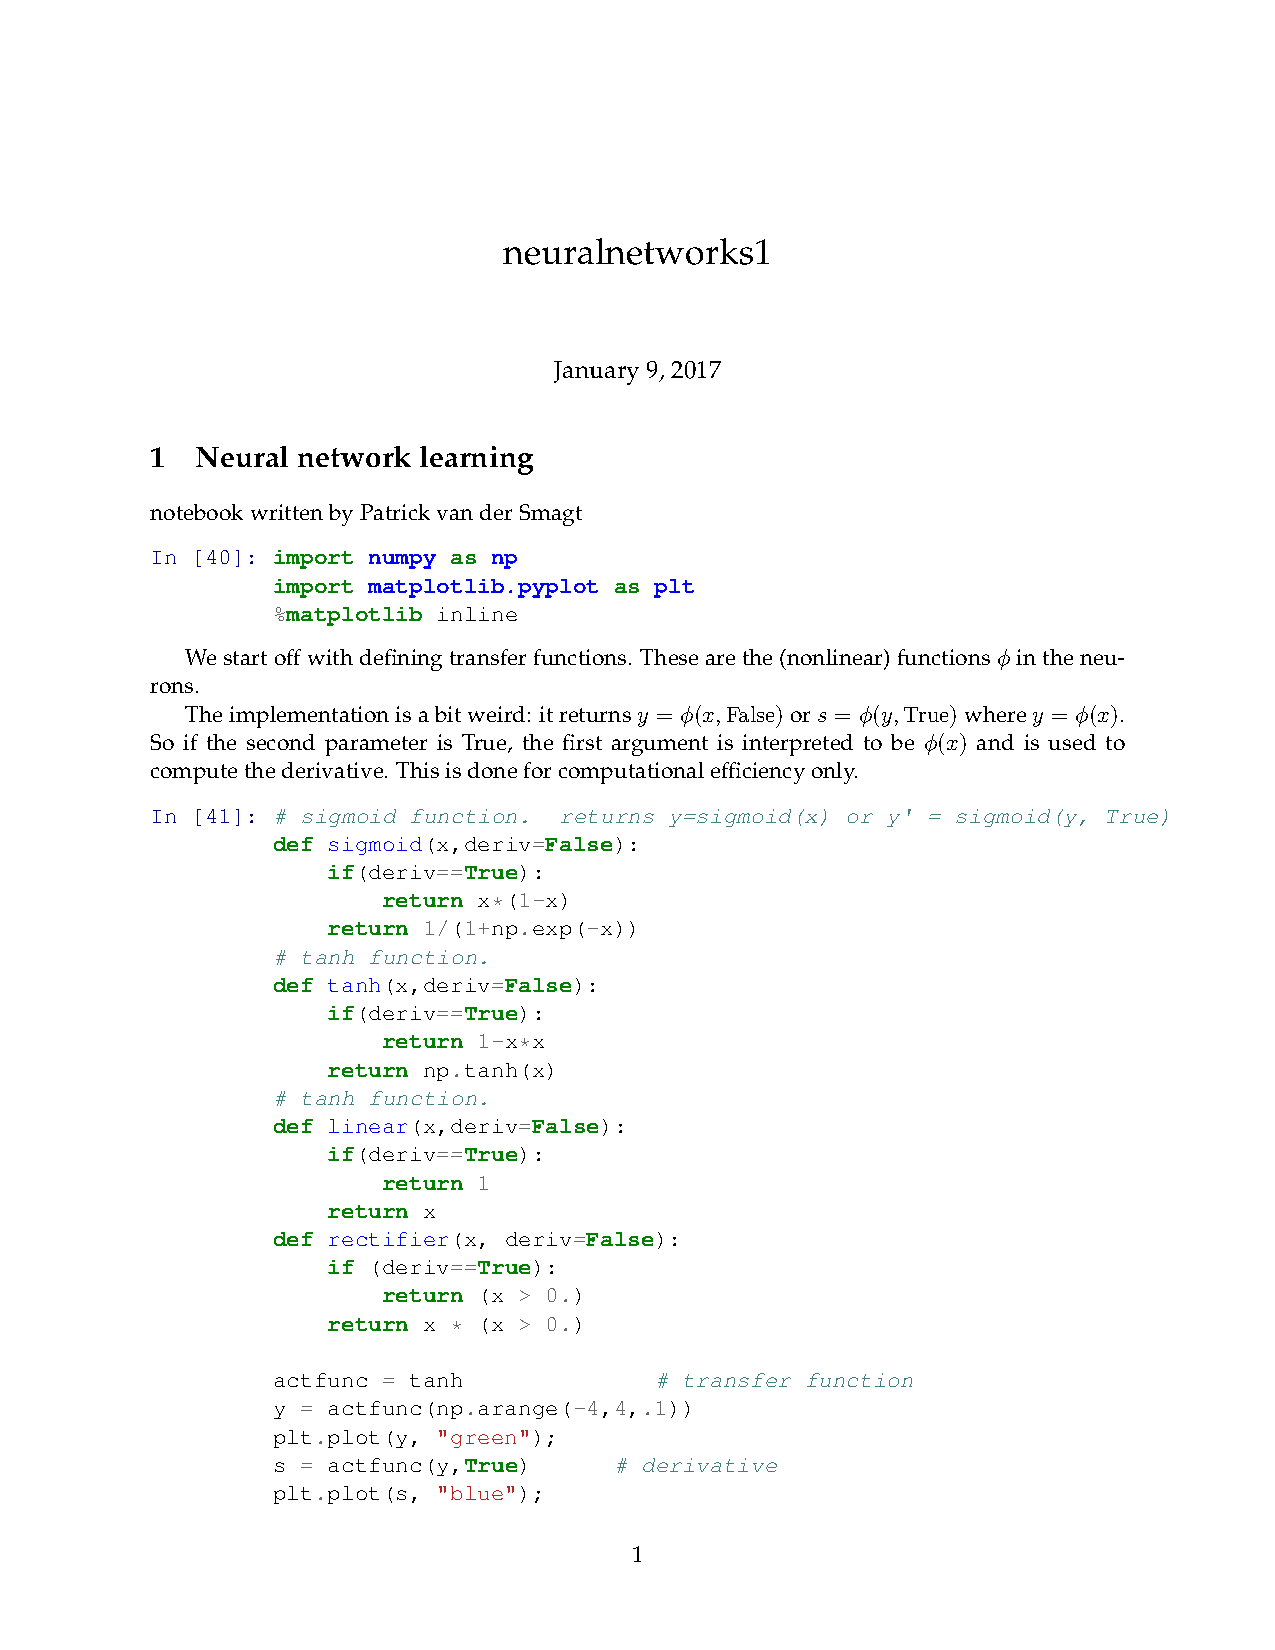
\includepdf[pages={1-7}]{neuralnetworks1.pdf}

\end{document}